\documentclass[10pt,twocolumn]{article}
\usepackage[a4paper, left=1.5cm, right=1.5cm, top=2cm, bottom=3cm]{geometry}
\usepackage[T1]{fontenc}
\usepackage[utf8]{inputenc}
\usepackage[italian]{babel}
\usepackage{amsmath}
\usepackage{titling}
\usepackage{caption}
\usepackage{graphicx}
\usepackage{float}
\usepackage{relsize}
\usepackage{amsmath}
\usepackage{sectsty}
\usepackage{ragged2e}
\usepackage{circuitikz}
\usepackage{booktabs}
\usepackage{enumitem}
\usepackage{tikz}
\usepackage{physics}
\usepackage{xcolor}
\usepackage[most]{tcolorbox}
\usepackage{tikz-3dplot}
\usepackage{tikz}
\usepackage{ragged2e}
\usepackage{siunitx}
% \usepackage{booktabs}
\usepackage[colorlinks=true, linkcolor=black]{hyperref}  %per rendere l'indice genrale "interattivo"
\usepackage{enumitem}  %distanza degli itemize
\setlist[itemize]{itemsep=4pt, parsep=1pt}
\newtcolorbox{nota}{
  blanker,
  before skip=1em,
  after skip=1em,
  left=1em,
  borderline west={1pt}{0pt}{black},
  fontupper=\itshape,
  before upper={\noindent\textbf{Nota}:\quad}
}



\begin{document}
\justifying
	\title{\textbf{Misura della curva caratteristica del diodo}}
	\author{Brusini Alessio \hspace{0.7cm} Ferrari Carola \hspace{0.7cm} Mirolo Manuele \hspace{0.7cm} Stroili Emanuele}
	\date{21 Ottobre 2025}
	\maketitle
	\newgeometry{left=3cm, right=3cm, top=4cm, bottom=4cm}
	\onecolumn
	\tableofcontents
\vspace{3cm}
	\begin{abstract}
		\centering
		\large
    L'esperimento consiste nell'ottenere la curva volt-amperometrica di una 
    lampadina a filamento, partendo da tensioni basse fino alla fusione del 
    tungsteno. L'obiettivo è verificare l'andamento non ohmico della resistenza
    interna della lampadina, 
       
	\end{abstract}

	\newpage
\restoregeometry
\twocolumn


\begin{figure}[H] % [h] = here, posizione approssimativa
  \centering
  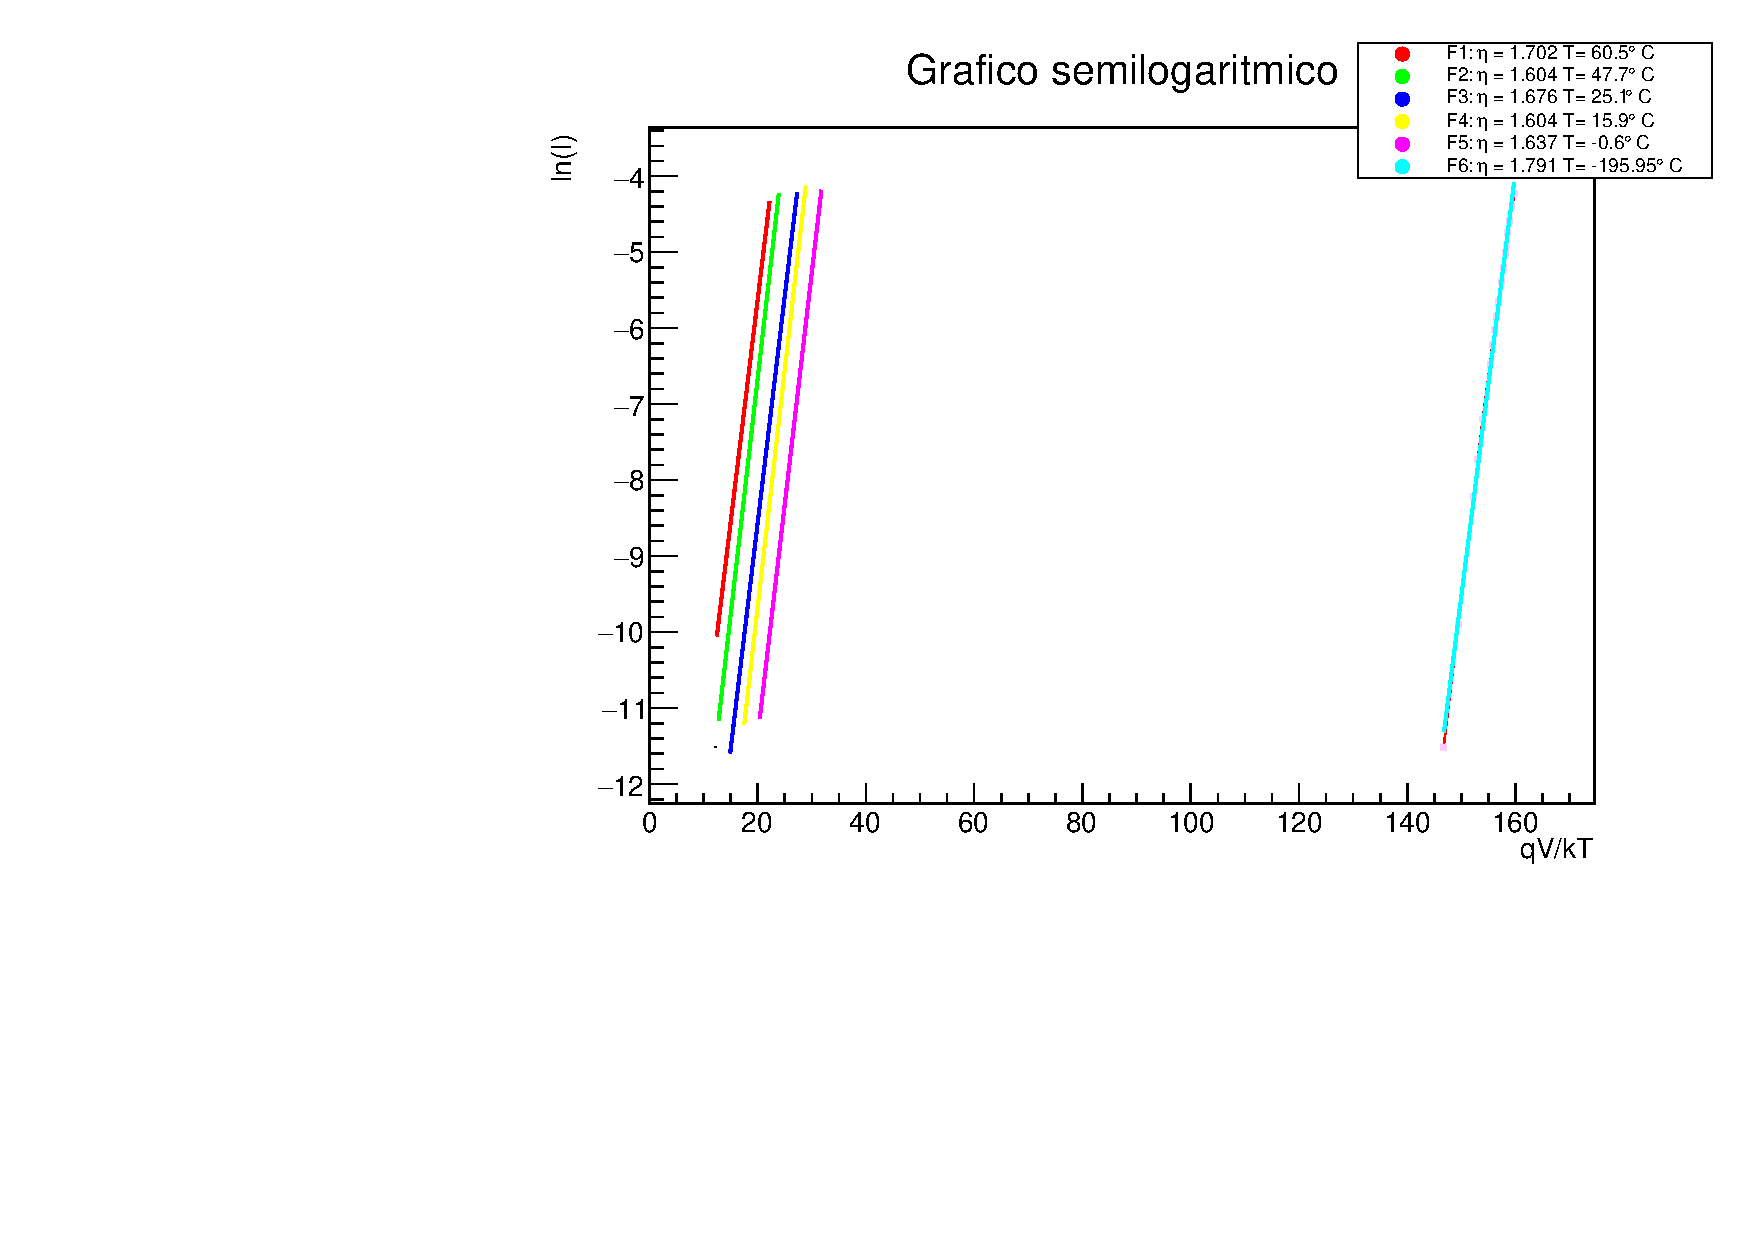
\includegraphics[width=0.5\textwidth]{coefficente_etatot.pdf} % o .png, .pdf, ecc.
  \label{fig:I}
\end{figure}
\begin{figure}[H] % [h] = here, posizione approssimativa
  \centering
  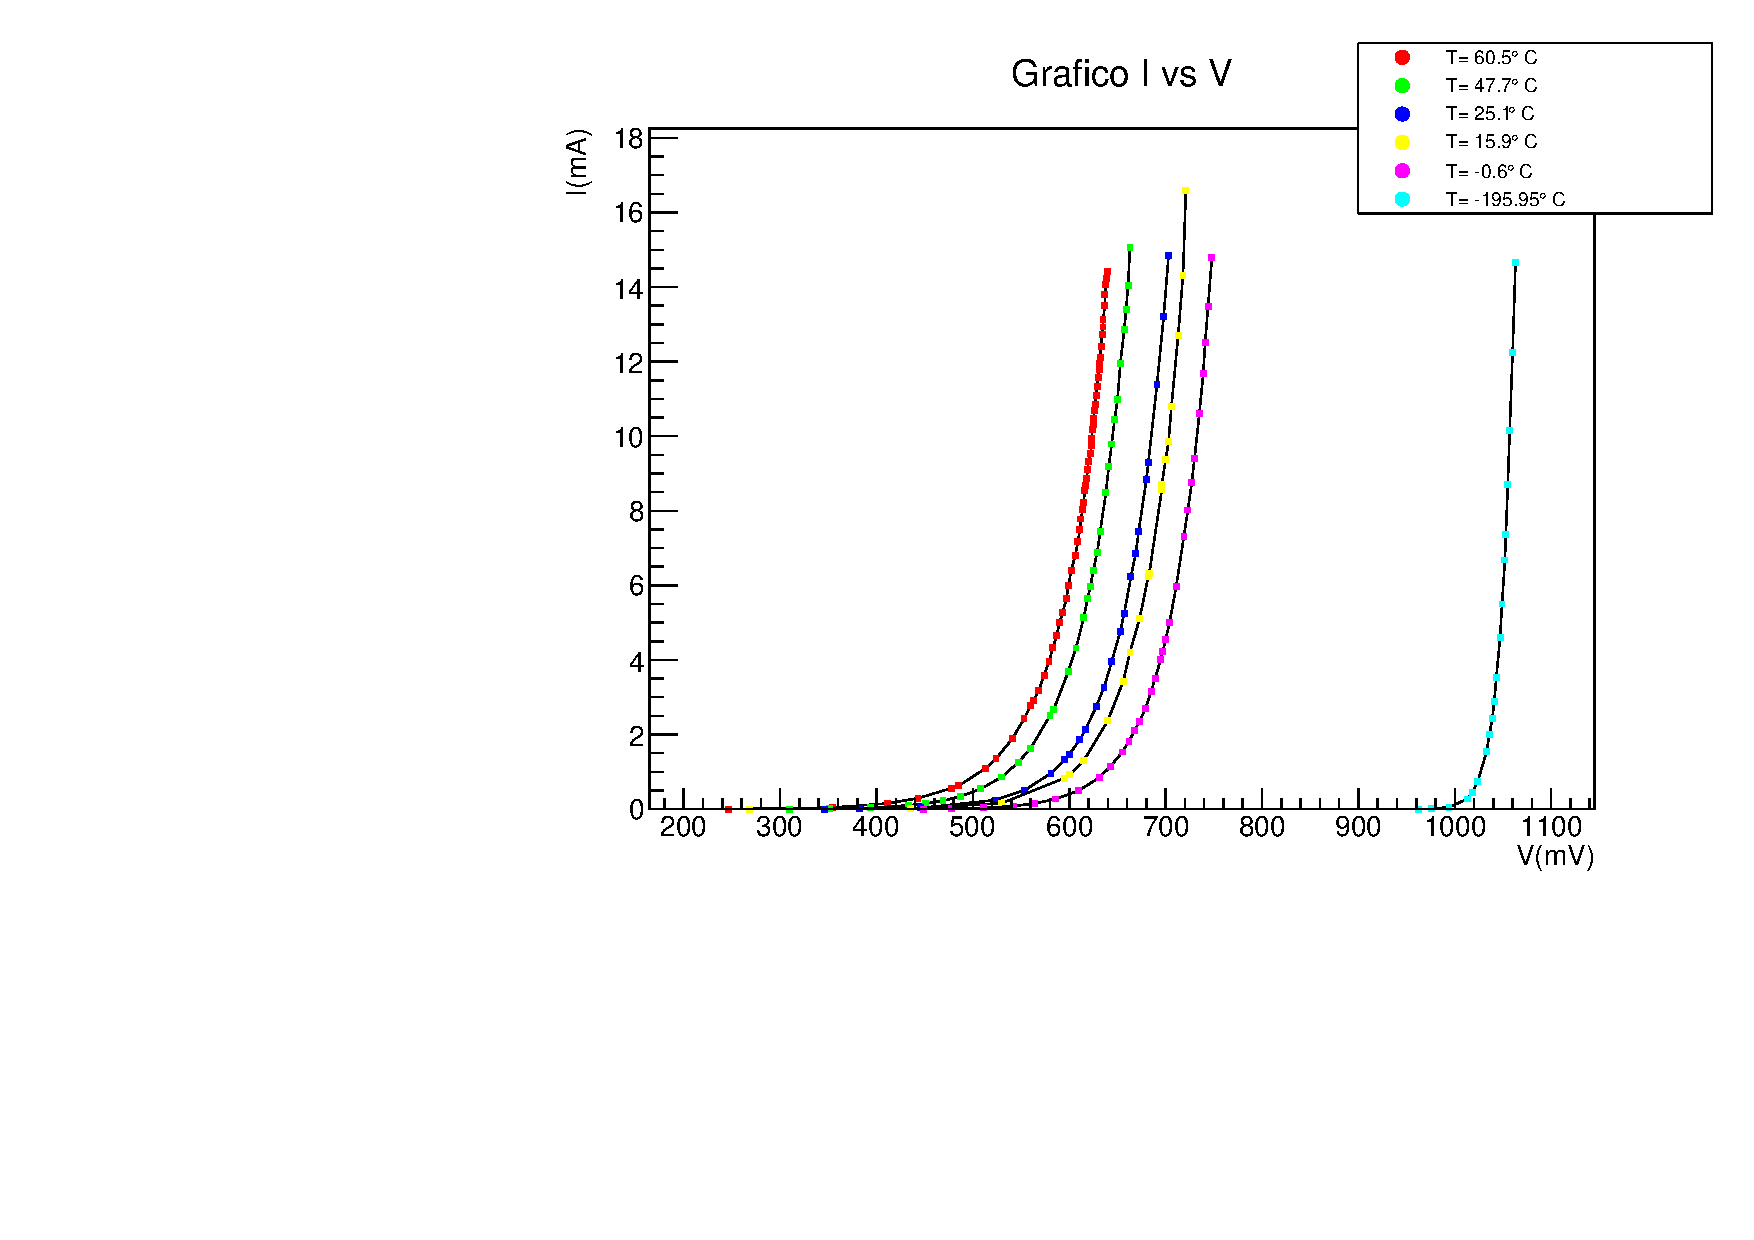
\includegraphics[width=0.5\textwidth]{I_vs_V.pdf.pdf} % o .png, .pdf, ecc.
  \label{fig:II}
\end{figure}
\begin{figure}[H] % [h] = here, posizione approssimativa
  \centering
  \includegraphics[width=0.5\textwidth]{log_I_vs_V.pdf} % o .png, .pdf, ecc.
  \label{fig:III}
\end{figure}
\begin{figure}[H] % [h] = here, posizione approssimativa
  \centering
  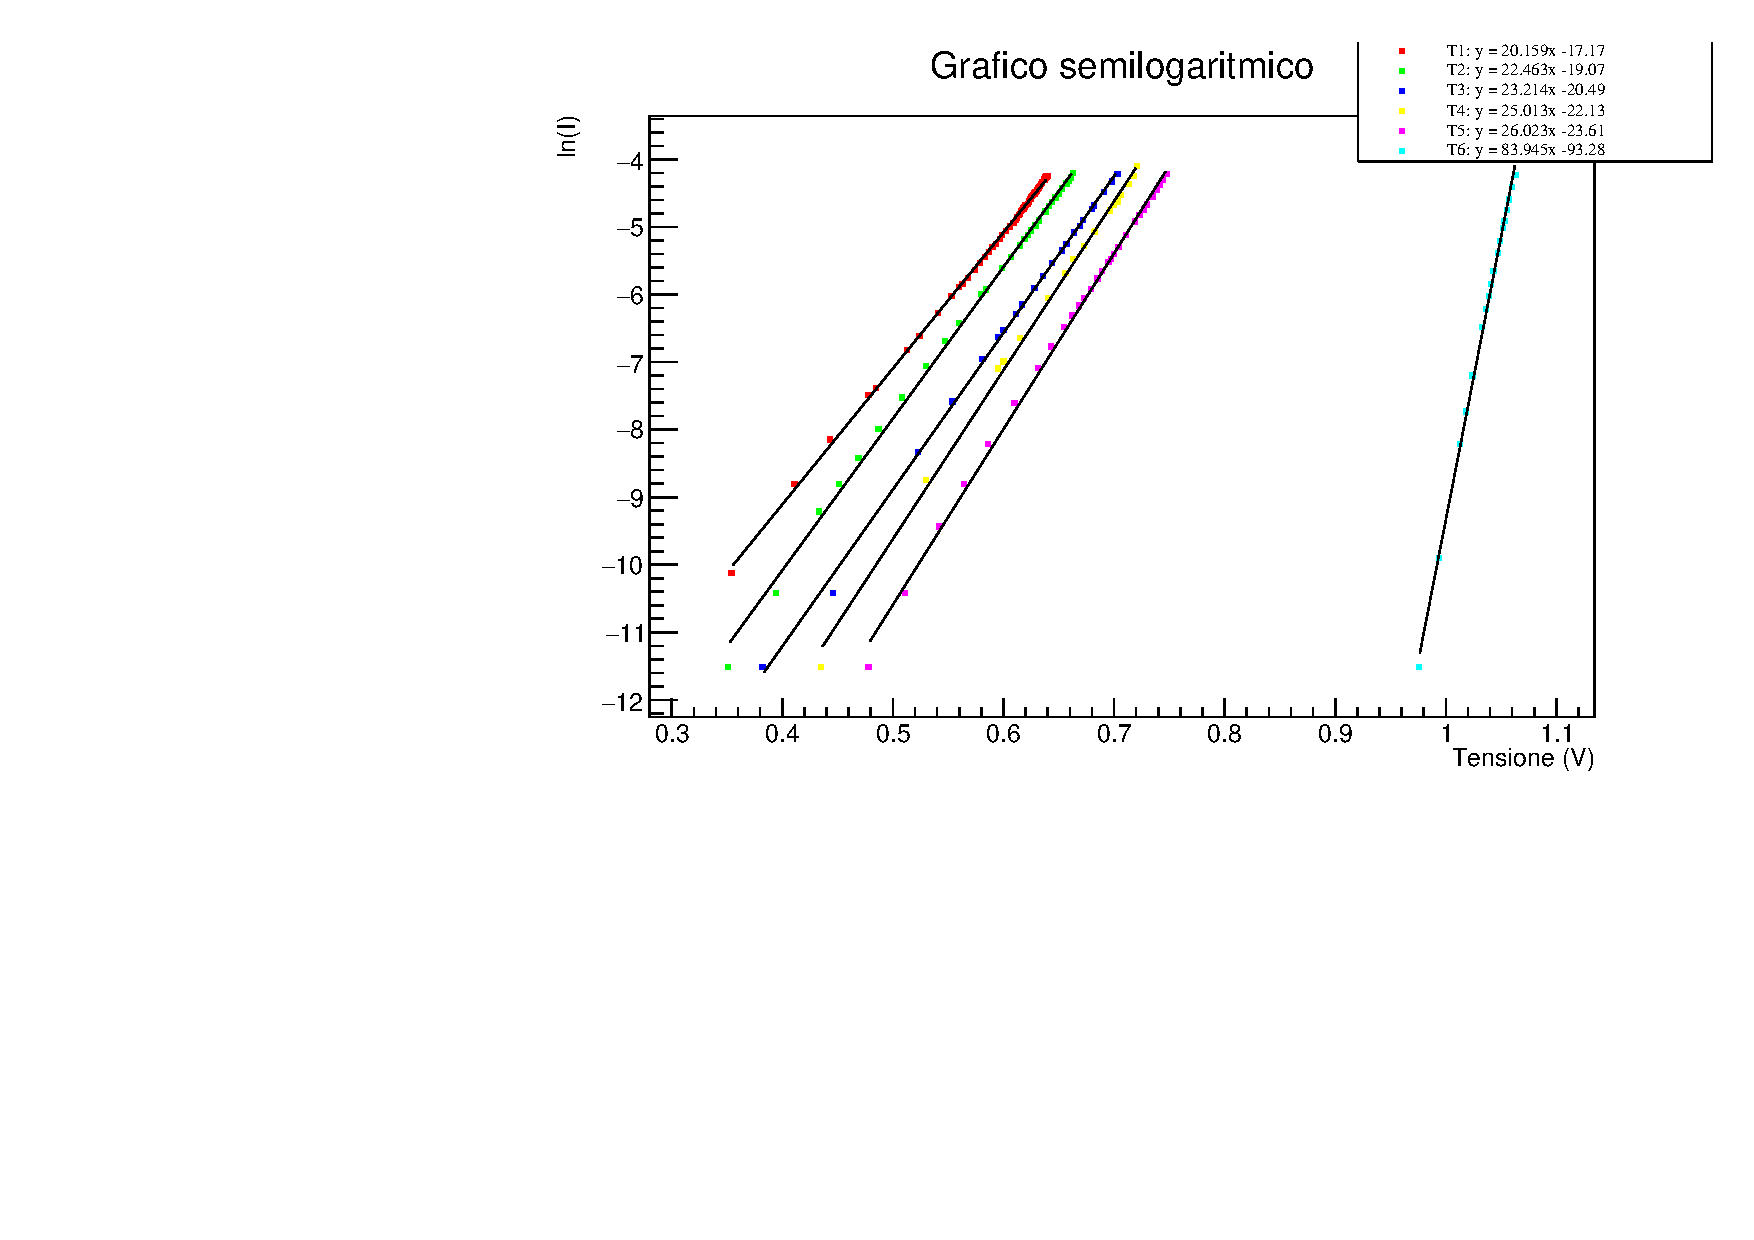
\includegraphics[width=0.5\textwidth]{scala_semilogaritmica.pdf} % o .png, .pdf, ecc.
  \label{fig:I_V_}
\end{figure}
\begin{figure}[H] % [h] = here, posizione approssimativa
  \centering
  \includegraphics[width=0.5\textwidth]{V_vs_I.pdf} % o .png, .pdf, ecc.
  \label{fig:V}
\end{figure}
\begin{figure}[H] % [h] = here, posizione approssimativa
  \centering
  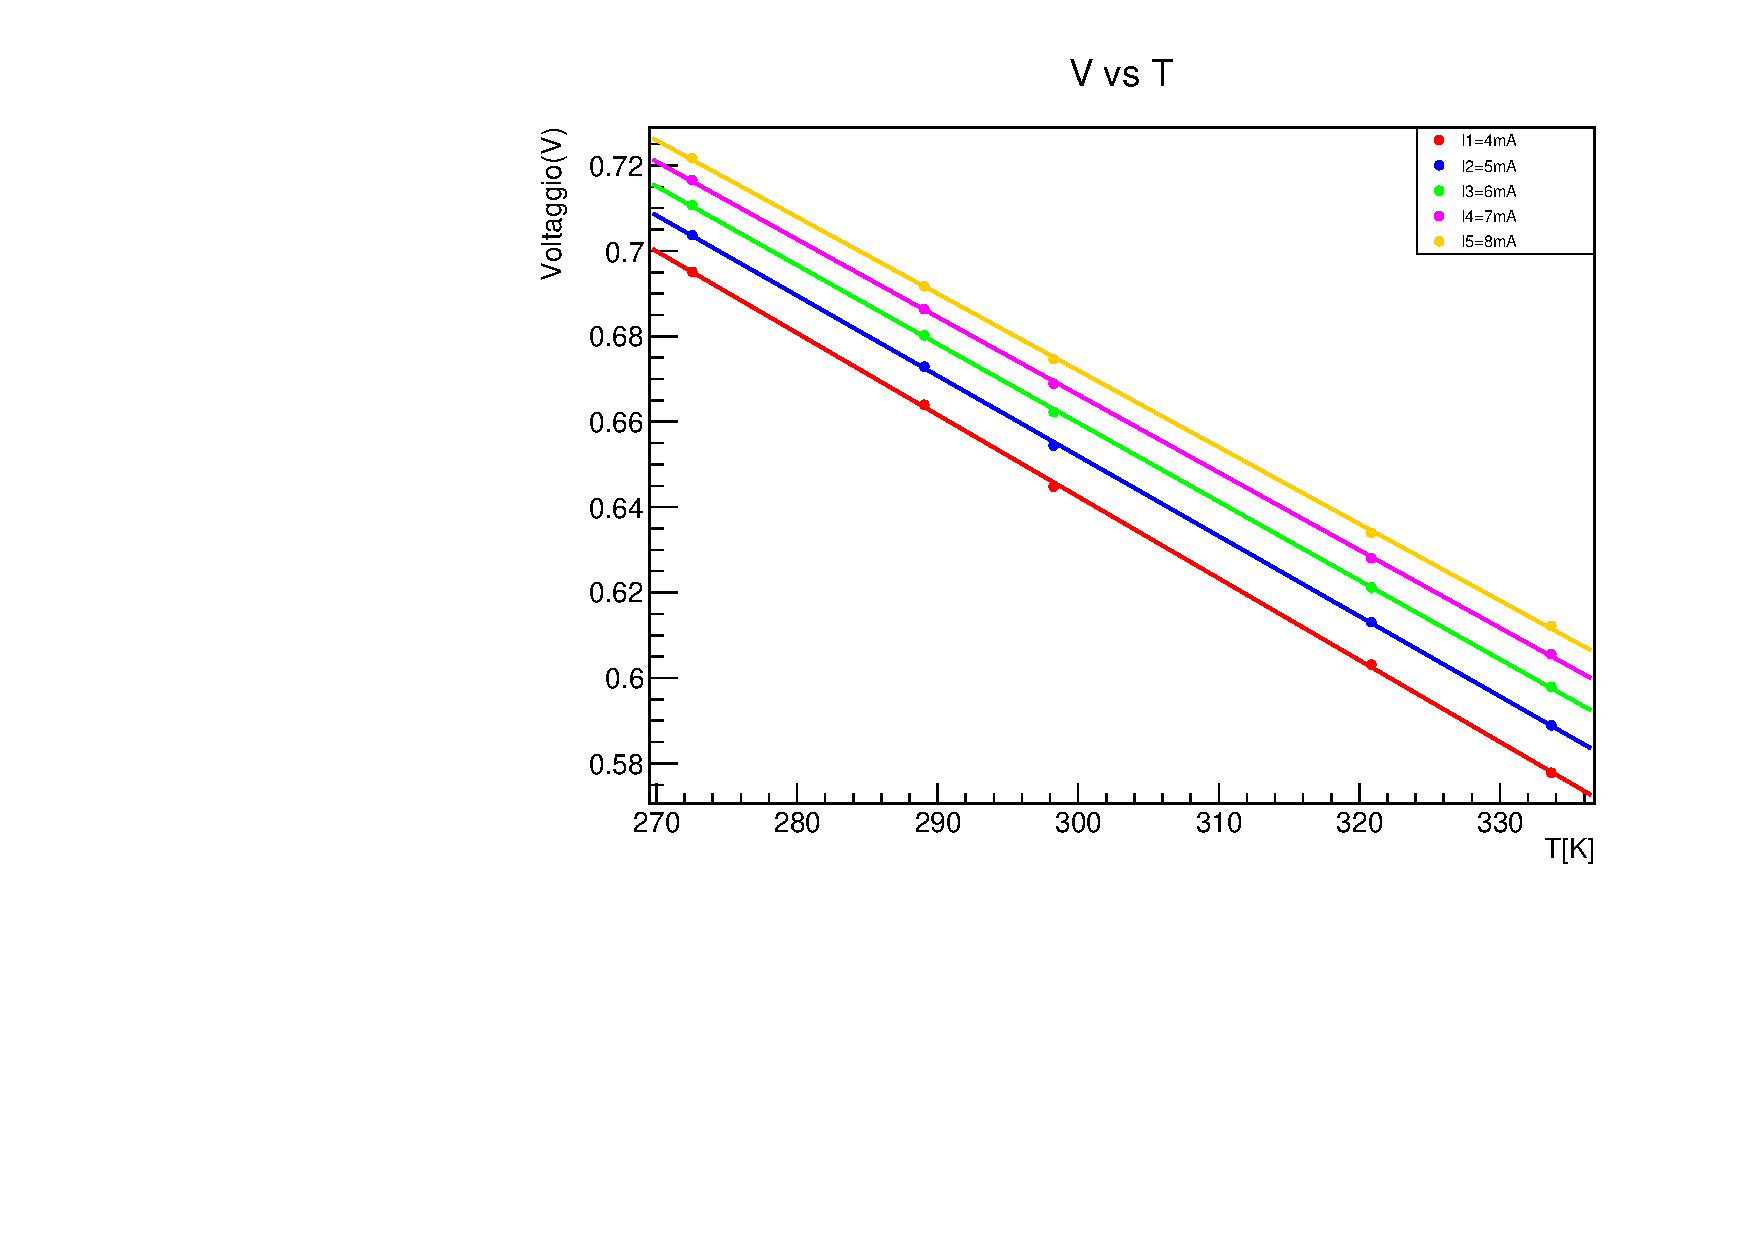
\includegraphics[width=0.5\textwidth]{V_vs_T_lim.pdf} % o .png, .pdf, ecc.
  \label{fig:V_I_}
\end{figure}
\end{document}